
\documentclass[cleanfoot]{asme2ej}

\usepackage[]{graphicx}
\graphicspath{ {images/} }

\usepackage{amsmath,amssymb}
\usepackage{textcomp}
\usepackage[urlcolor=blue,linkcolor=red,colorlinks=true]{hyperref}
\usepackage[autostyle, english=american]{csquotes}
\MakeOuterQuote{"}

\title{Exoplanet Open-Source Imaging Mission Simulator (EXOSIMS) \\ Interface Control Document}

%%% first author
\author{Daniel Garrett and Dmitry Savransky
    \affiliation{
    Sibley School of Mechanical and Aerospace Engineering\\
	Cornell University\\
	Ithaca, NY 14853
    }	
}


\begin{document}

\maketitle    

%%%%%%%%%%%%%%%%%%%%%%%%%%%%%%%%%%%%%%%%%%%%%%%%%%%%%%%%%%%%%%%%%%%%%%
\begin{abstract}
{\it This document describes the extensible, modular, open source software framework EXOSIMS.  EXOSIMS creates end-to-end simulations of space-based exoplanet imaging missions using stand-alone software modules.  These modules are split into input and simulation module groups.  The input/output interfaces of each module and interactions of modules with each other are presented to give guidance on mission specific modifications to the EXOSIMS framework.}
\end{abstract}

\tableofcontents

%%%%%%%%%%%%%%%%%%%%%%%%%%%%%%%%%%%%%%%%%%%%%%%%%%%%%%%%%%%%%%%%%%%%%%
\begin{nomenclature}
\entry{EXOSIMS}{Exoplanet Open-Source Imaging Mission Simulator}
\entry{HE}{Heliocentric Equatorial}
\entry{ICD}{Interface Control Document}
\entry{MJD}{Modified Julian Day}
\entry{OD}{Observatory Definition}
\entry{OSD}{Optical System Description}
\entry{PP}{Post-Processing}
\entry{PPD}{Planet Population Description}
\entry{PPM}{Planet Physical Model}
\entry{SC}{Star Catalog}
\entry{SE}{Survey Ensemble}
\entry{SS}{Survey Simulation}
\entry{SU}{Simulated Universe}
\entry{TL}{Target List}
\entry{ZL}{Zodiacal Light}
\end{nomenclature}

%%%%%%%%%%%%%%%%%%%%%%%%%%%%%%%%%%%%%%%%%%%%%%%%%%%%%%%%%%%%%%%%%%%%%%
% INTRODUCTION
%%%%%%%%%%%%%%%%%%%%%%%%%%%%%%%%%%%%%%%%%%%%%%%%%%%%%%%%%%%%%%%%%%%%%%

\section{Introduction} 
Building confidence in a mission concept's ability to achieve its science goals is always desirable.  Unfortunately, accurately modeling the science yield of an exoplanet imager can be almost as complicated as designing the mission.  It is challenging to compare science simulation results and systematically test the effects of changing one aspect of the instrument or mission design.

EXOSIMS (Exoplanet Open-Source Imaging Mission Simulator) addresses this problem by generating ensembles of mission simulations for exoplanet direct imaging missions to estimate science yields. It is designed to allow systematic exploration of exoplanet imaging mission science yields.  It consists of stand-alone modules written in Python which may be modified without requiring modifications to other portions of the code. This allows EXOSIMS to be easily used to investigate new designs for instruments, observatories, or overall mission designs independently. This document describes the required input/output interfaces for the stand-alone modules to enable this flexibility.

\subsection{Purpose and Scope} % Rework this section
This Interface Control Document (ICD) provides an overview of the software framework of EXOSIMS and some details on its component parts.  As the software is intended to be highly reconfigurable, operational aspects of the code are emphasized over implementational details.  Specific examples are taken from the coronagraphic instrument under development for WFIRST-AFTA.  The data inputs and outputs of each module are described. Following these guidelines will allow the code to be updated to accommodate new mission designs.

This ICD defines the input/output of each module and the interfaces between modules of the code.  This document is intended to guide mission planners and instrument designers in the development of specific modules for new mission designs.

%\subsection{Glossary}
%This section will contain definition of terms used throughout the document if needed.

%%%%%%%%%%%%%%%%%%%%%%%%%%%%%%%%%%%%%%%%%%%%%%%%%%%%%%%%%%%%%%%%%%%%%%%%%
% OVERVIEW 
%%%%%%%%%%%%%%%%%%%%%%%%%%%%%%%%%%%%%%%%%%%%%%%%%%%%%%%%%%%%%%%%%%%%%%%%%

\section{Overview}
The terminology used to describe the software implementation is loosely based on the object-oriented Python framework upon which EXOSIMS is built.  The term module can refer to the object class prototype representing the abstracted functionality of one piece of the software, an implementation of this object class which inherits the attributes of the prototype, or an instance of this object class.  Input/output definitions of modules refer to the class prototype.  Implemented modules refer to the inherited class definition.  Passing modules (or their outputs) means the instantiation of the inherited object class being used in a given simulation.  Relying on strict inheritance for all implemented module classes provides an automated error and consistency-checking mechanism.  The outputs of a given object instance may be compared to the outputs of the prototype.  It is trivial to pre-check whether a given module implementation will work with the larger framework, and thus allows flexibility and adaptability.

\begin{figure}[ht]
    \begin{center}
        \begin{tabular}{c}
             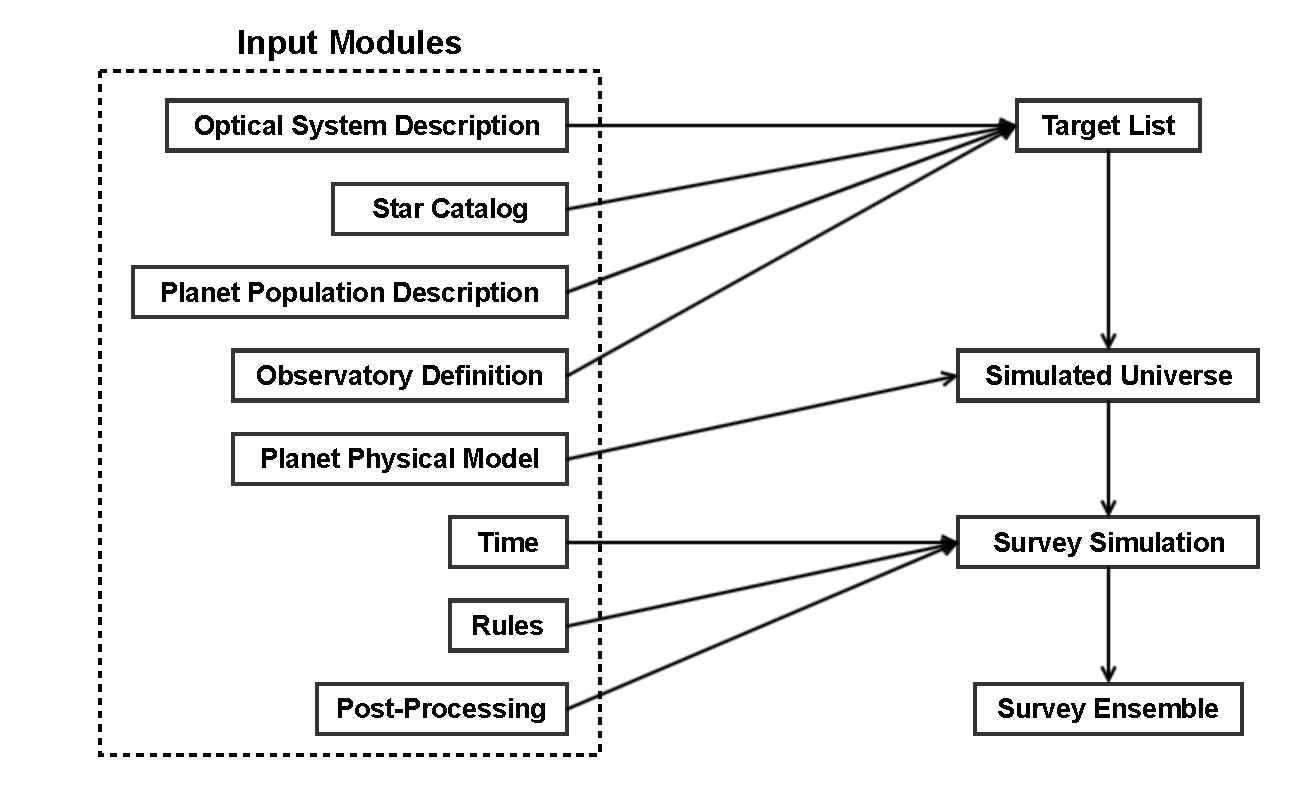
\includegraphics[width=\textwidth]{codeflow2}
        \end{tabular}
    \end{center}
    \caption{Flowchart of mission simulation. Each box represents a component software module which interacts with other modules as indicated by the arrows. The simulation modules (those that are not classified as input modules) pass all input modules along with their own output.  Thus, the Survey Ensemble module has access to all of the input modules and all of the upstream simulation modules.}
    \label{figure_framework}
\end{figure}

The overall framework of EXOSIMS is depicted in Fig.~\ref{figure_framework} where the component stand-alone software modules are classified as input modules and simulation modules.  The input modules include the Optical System Description (OSD), Star Catalog (SC), Planet Population Description (PPD), Observatory Definition (OD), Planet Physical Model (PPM), Time, Rules, and Post-Processing (PP) modules.  These modules contain specific mission design parameters.  The simulation modules include Target List (TL), Simulated Universe (SU), Survey Simulation (SS), and Survey Ensemble (SE) modules.  The simulation modules take information contained in the input modules and perform mission simulation tasks.  Any module may perform any number or kind of calculations using any or all of the input parameters provided.  They are only constrained by their input and output specification contained in this document.

\begin{figure}[ht]
    \begin{center}
        \begin{tabular}{c}
             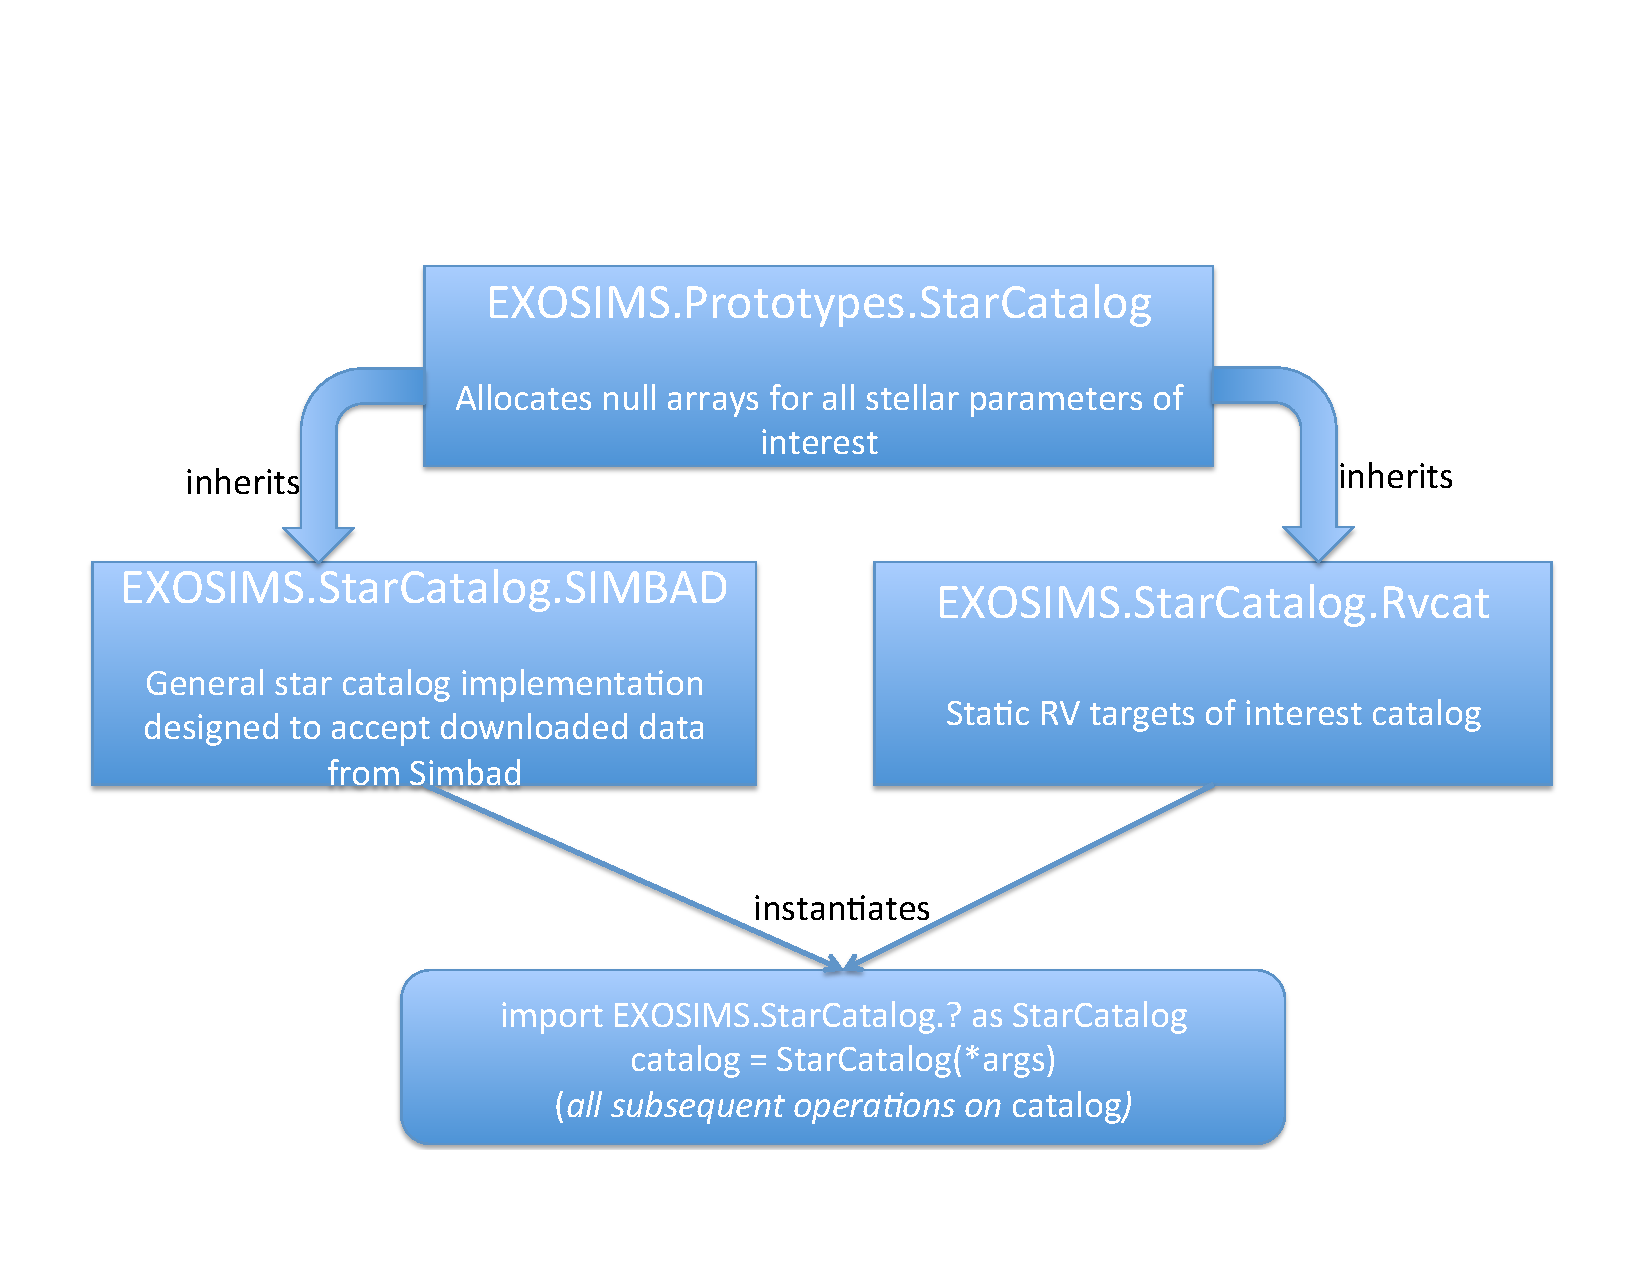
\includegraphics[width=0.75\textwidth]{starcatalog_flowdown}
        \end{tabular}
    \end{center}
    \caption{Schematic of a sample implementation for the three module layers for the Star Catalog module. The Star Catalog prototype (top row) is immutable, specifies the input/output structure of the module along with all common functionality, and is inherited by all Star Catalog class implementations (middle row).  In this case, two different catalog classes are shown: one that reads in data from a SIMBAD catalog dump, and one which contains only information about a subset of known radial velocity targets.  The object used in the simulation (bottom row) is an instance of one of these classes, and can be used in exactly the same way in the rest of the code due to the common input/output scheme.}
    \label{fig:starcatalog_flowdown}
\end{figure}

\begin{figure}[ht]
    \begin{center}
        \begin{tabular}{c}
             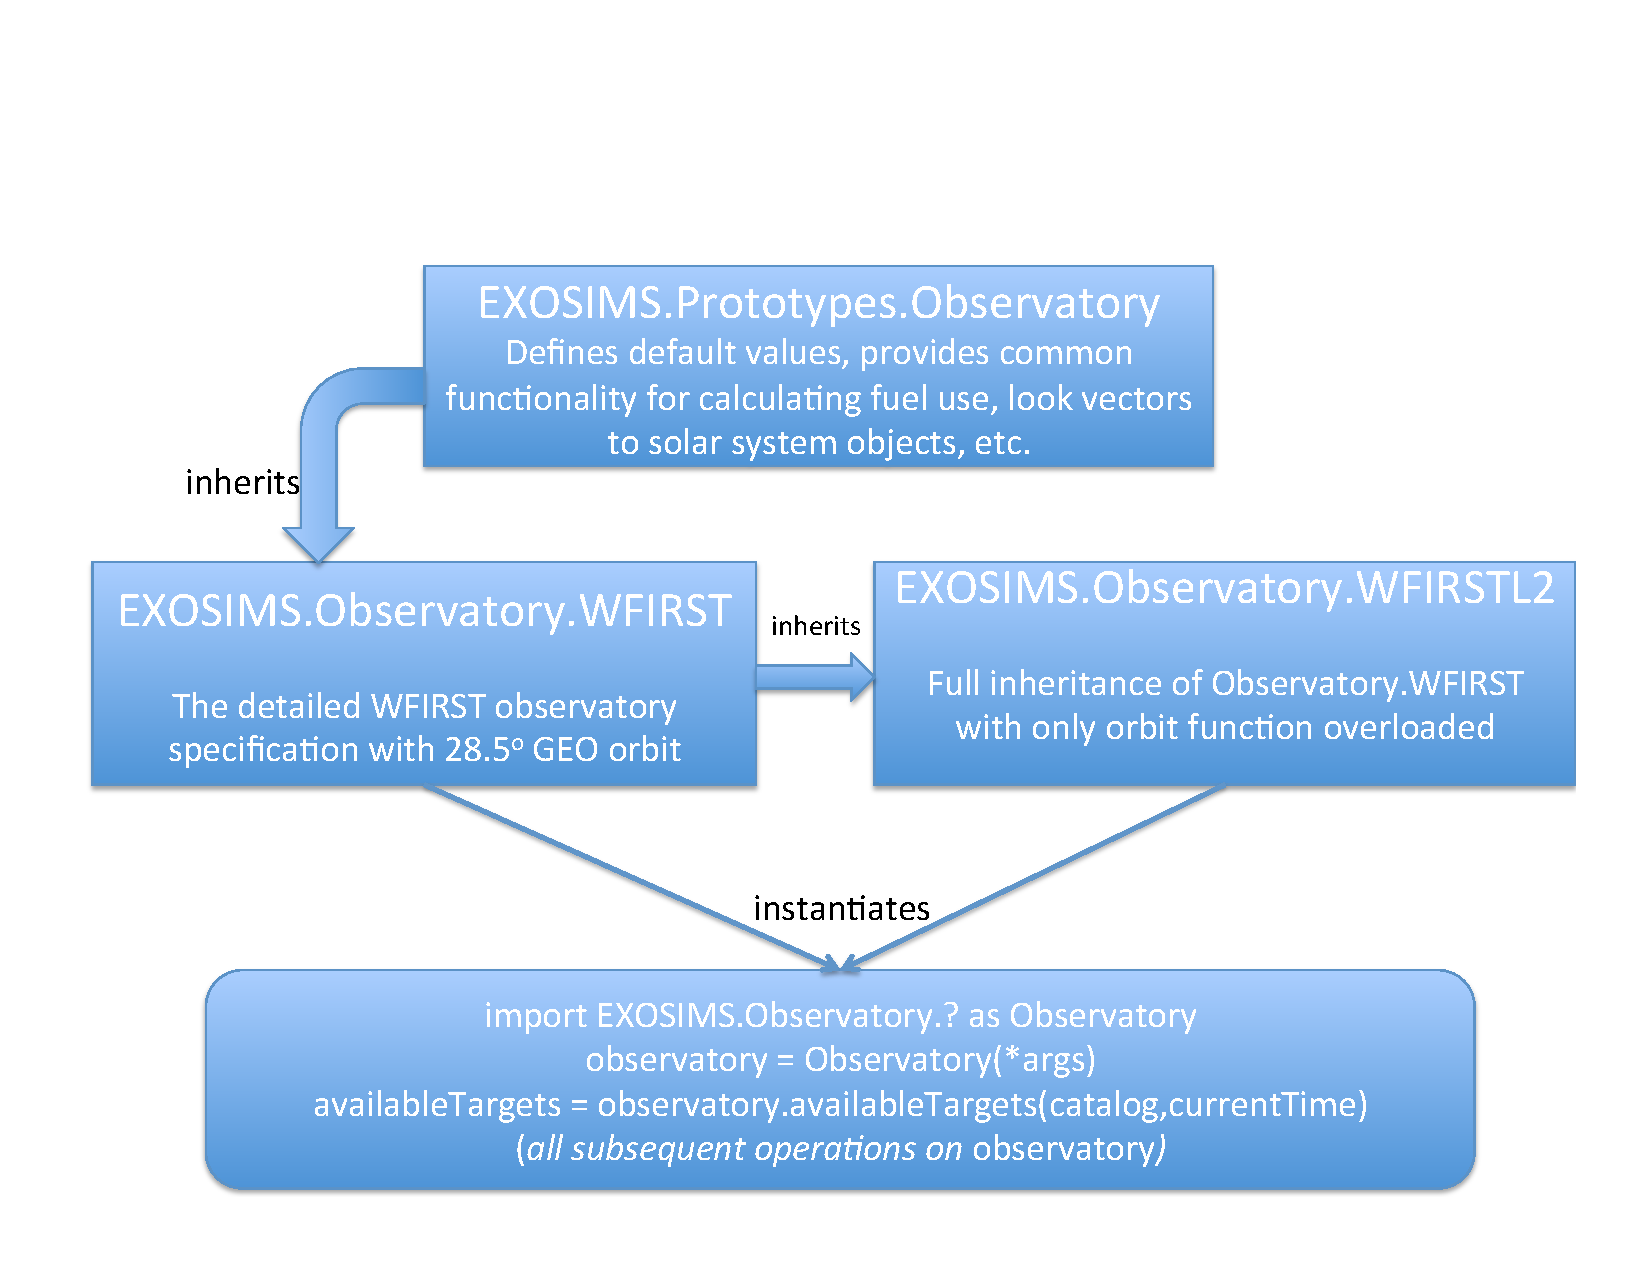
\includegraphics[width=0.75\textwidth]{observatory_flowdown}
        \end{tabular}
    \end{center}
    \caption{Schematic of a sample implementation for the three module layers for the Observatory Description module. The Observatory Definition prototype (top row) is immutable, specifies the input/output structure of the module along with all common functionality, and is inherited by all Observatory Definition class implementations (middle row).  In this case, two different observatory classes are shown that differ only in the definition of the observatory orbit.  Therefore, the second implementation inherits the first (rather than directly inheriting the prototype) and overloads only the orbit method. The object used in the simulation (bottom row) is an instance of one of these classes, and can be used in exactly the same way in the rest of the code due to the common input/output scheme.}
    \label{fig:observatory_flowdown}
\end{figure}

Figures \ref{fig:starcatalog_flowdown} and \ref{fig:observatory_flowdown} show schematic representations of the three different apsects of a module, for the Star Catalog and Observatory Definition modules, respectively.  Every module has a specific prototype that sets the input/output structure of the module and encodes any common functionality for all module class implementations.  The various implementations inherit the prototype and perform whatever processing is necessary, limited only by the preset input/output scheme.  Finally, in the course of running a simulation, an object is generated for each module class selected for that simulation.  The generated objects can be used in exactly the same way in the downstream code, regardless of what implementation they are instances of, due to the strict interface defined in the class prototypes.

For the input modules, the input specification is much more loosely defined than the output specification, as different implementations may draw data from a wide variety of sources.  For example, the star catalog may be implemented as reading values from a static file on disk, or may represent an active connection to a local or remote database.  The output specification for these modules, however, as well as both the input and output for the simulation modules, is entirely fixed so as to allow for generic use of all module objects in the simulation.

%%%%%%%%%%%%%%%%%%%%%%%%%%%%%%%%%%%%%%%%%%%%%%%%%%%%%%%%%%%%%%%%%%%%%%%%%
% GLOBAL SPECIFICATIONS (INCLUDE BETTER EXPLANATIONS)
%%%%%%%%%%%%%%%%%%%%%%%%%%%%%%%%%%%%%%%%%%%%%%%%%%%%%%%%%%%%%%%%%%%%%%%%%

\section{Global Specifications}
Common references (units, frames of reference, etc.) are required to ensure interoperability between the modules of EXOSIM.  All of the references listed below must be followed.

\begin{description}
    \item[Common Epoch] \hfill \\ J2000
    \item[Common Reference Frame] \hfill \\ Heliocentric Equatorial (HE)
    \item[Common Time] \hfill \\ Modified Julian Day (MJD $\triangleq$ JD - 2400000.5)
\end{description}

\subsection{Python Packages} 
EXOSIMS is an open source platform.  As such, packages and modules may be imported and used for calculations within any of the stand-alone modules.  The following commonly used Python packages are used for the WFIRST-specific implementation of EXOSIMS:

\texttt{
\begin{itemize}
    \item astropy
        \begin{itemize}
            \item astropy.constants
            \item astropy.coordinates
            \item astropy.time
            \item astropy.units
        \end{itemize}
    \item importlib
    \item numpy
        \begin{itemize}
            \item numpy.linalg 
        \end{itemize}
    \item os
        \begin{itemize}
            \item os.path 
        \end{itemize}
    \item pickle/cPickle
    \item scipy
        \begin{itemize}
            \item scipy.io
            \item scipy.special
        \end{itemize}
\end{itemize}
}
%%%%%%%%%%%%%%%%%%%%%%%%%%%%%%%%%%%%%%%%%%%%%%%%%%%%%%%%%%%%%%%%%%%%
% BACKBONE
%%%%%%%%%%%%%%%%%%%%%%%%%%%%%%%%%%%%%%%%%%%%%%%%%%%%%%%%%%%%%%%%%%%%

\section{Backbone}
All simulation execution will be performed by the backbone.  This set of functions will have very limited built-in functionality, and will primarily be tasked with parsing the input specification described below, and then calling the specified instances of each of the framework modules, detailed in \S\ref{sec:modules}.

A simulation specification is a single JSON-formatted (\url{http://json.org/}) file that encodes user-settable parameters and module names.  The backbone will contain a reference specification with \emph{all} parameters and modules set.  In the initial parsing of the user-supplied specification, it will be merged with the reference specification such that any fields not set by the user will be assigned to their reference (default) values. 

The backbone will contain a standalone specification parser that will check specification files for internal consistency.  For example, if modules carry mutual dependencies, the specification parser will return an error if these are not met for a given specification.  Similarly, if modules are selected with optional top level inputs, warnings will be generated if these are not set in the same specification files.

The backbone will contain an interactive function to help users generate specification files via a series of questions.

\subsection{Specification Format}
\begin{verbatim}
{
  "missionLifetime": 6,
  "missionDutyCycle": 0.24,
  "starlightSupressionSystems": [
    {
      "type": "SDO",
      "occulterDiameter": 50,
      "occulterDistance": 50000,
      "PSFfile": "/data/sdo1_psf.fits",
      "throughputFile": "/data/sdo1_thru.fits"
    },
    {
      "type": "coronagraph",
      "IWA": 3,
      "PSFfile": "/data/coron1_psf.fits",
      "throughputFile": "/data/coron1_thru.fits"
    }
  ],
  OSDmod: "hybridOSD1"
}
\end{verbatim}

%%%%%%%%%%%%%%%%%%%%%%%%%%%%%%%%%%%%%%%%%%%%%%%%%%%%%%%%%%%%%%%%%%%%%%%%%
% INPUT MODULES DESCRIPTION
%%%%%%%%%%%%%%%%%%%%%%%%%%%%%%%%%%%%%%%%%%%%%%%%%%%%%%%%%%%%%%%%%%%%%%%%%

\section{Input Modules}\label{sec:modules}
The input modules include Optical System Description (OSD), Star Catalog (SC), Planet Population Description (PPD), Observatory Definition (OD), Planet Physical Model (PPM), Time, Rules, and Post-Processing (PP).  These modules encode and/or generate all of the information necessary to perform mission simulations.  The specific mission design determines the functionality of each input module, while inputs and outputs of these modules remain the same (in terms of data type and variable representations).  This section defines the functionality, major tasks, input, output, and interface of each of these modules.

% OPTICAL SYSTEM DESCRIPTION NEEDS UPDATING

\subsection{Optical System Description (OSD) NEEDS UPDATING}
The OSD module contains all of the necessary information to describe the effects of the telescope and starlight suppression system on the target star and planet wavefronts.  This requires encoding the design of both the telescope optics and the specific starlight suppression system, whether it be an internal coronagraph or an external occulter.  The encoding can be achieved by specifying Point Spread Functions (PSF) for on- and off-axis sources, along with (potentially angular separation-dependent) contrast and throughput definitions.  At the opposite level of complexity, the encoded portions of this module may be a description of all of the optical elements between the telescope aperture and the imaging detector, along with a method of propagating an input wavefront to the final image plane.  Intermediate implementations can include partial propagations, or collections of static PSFs representing the contributions of various system elements.  The encoding of the optical train will allow for the extraction of specific bulk parameters including the instrument inner working angle (IWA), outer working angle (OWA), and mean and max contrast and throughput.

Finally, the OSD must also include a description of the science instrument.  The baseline instrument is assumed to be an imaging spectrometer.  The encoding must provide the spatial and wavelength coverage of the instrument as well as sampling for each, along with detector details such as read noise, dark current, and readout cycle.

TASKS:


\label{sec:opticalsystem}
\subsubsection{Optical System Object Attribute Initialization Input/Output Description} 
\subsubsection*{Inputs}
\begin{itemize}
    \item
    \begin{description}
        \item[User specification] \hfill \\
        Information from simulation specification JSON file organized into a Python dictionary. If the below key: value pairs are missing from the dictionary, the Optical System object attributes will be assigned the default values listed.
        \begin{description}
            \item specs["lam"] \hfill \\
            Central or detection wavelength in $ nm $. Default value is 500.
            \item specs["shapeFac"] \hfill \\
            Shape factor so that $ shapeFac \times diameter^2 = Area $. Default value is $ \frac{\pi}{4} $.
            \item specs["pupilArea"] \hfill \\
            Entrance pupil area in $ m^2 $. Default value is $ 4\pi $.
            \item specs["SNchar"] \hfill \\
            Signal to Noise Ratio for characterization. Default value is 11.
            \item specs["haveOcculter"] \hfill \\
            Boolean signifying if system includes an occulter. Default value is False.
            \item specs["pixelArea"] \hfill \\
            Pixel area in $ m^2 $. Default value is 1e-10.
            \item specs["focalLength"] \hfill \\
            Focal length in $ m $. Default value is 240.
            \item specs["IWA"] \hfill \\
            Inner Working Angle in $ arcseconds $. Default value is 0.075.
            \item specs["OWA"] \hfill \\
            Outer Working Angle in $ arcseconds $. Default value is inf.
            \item specs["dMagLim"] \hfill \\
            Limiting $ \Delta$mag (difference in magnitude between star and planet). Default value is 26.
            \item specs["throughput"] \hfill \\
            Optical system throughput. Default value is 0.5. This may be a floating point scalar (representing a fixed throughput) or a \verb+scipy.interpolate.interp1d+ object representing variable throughput as a function of angular separation.  In the case of the latter, the interpolant must be valid between the IWA and the OWA, inclusive, and must assume an argument in arcseconds.
            \item specs["contrast"] \hfill \\
            Optical system suppression level at IWA. Default value is 1e-10. This may be a floating point scalar (representing a fixed contrast) or a \verb+scipy.interpolate.interp1d+ object representing variable contrast as a function of angular separation.  In the case of the latter, the interpolant must be valid between the IWA and the OWA, inclusive, and must assume an argument in arcseconds.
            \item specs["dr"] \hfill \\
            Detector dark current rate per pixel. Default value is 0.001.
            \item specs["sigma\_r"] \hfill \\
            Detector read noise. Default value is 3.
            \item specs["t\_exp"] \hfill \\
            Exposure time per read in $ s $. Default value is 1000.
            \item specs["QE"] \hfill \\
            Detector quantum efficiency. Default value is 0.5. This may be a floating point scalar (representing a fixed QE) or a \verb+scipy.interpolate.interp1d+ object representing variable QE as a function of wavelength.  In the case of the latter, the interpolant must be valid between the minimum and maximum wavelengths of the instrument (as defined by lambda and deltaLambda), inclusive, and must assume an argument in nanometers.
            \item specs["eta2"] \hfill \\
            Post coronagraph attenuation. Default value is 0.57.
            \item specs["deltaLambda"] \hfill \\
            Detection bandwidth $ \Delta\lambda $ in $ nm $. Default value is 100.
            \item specs["PSF"] \hfill \\
            Instrument point spread function stored as 2D numpy ndarray.  The core of the PSF should be normalized to 1, so that all throughput terms are combined in the througput variable above.
            \item specs["PSFsampling"] \hfill \\
            Sampling of the PSF in arcsec/pixel.
        \end{description}
    \end{description}
\end{itemize}

For all values that may be either scalars or interpolants, in the case where scalar values are given, the optical system module will automatically wrap them in lambda functions so that they become callable (just like the interpolant) but will always return the same value for all arguments.  The inputs for interpolants may be filenames with tabulated data, or numpy ndarrays of argument and data (in that order in rows so that input[0] is the argument and input[1] is the data).

\subsubsection*{Outputs}
\begin{itemize}
    \item 
    \begin{description}
        \item[OpticalSys.lam] \hfill \\
        Central or detection wavelength (astropy unit object initially defined in nm)
        \item[OpticalSys.shapeFac] \hfill \\
        Shape factor so that $ shapeFac \times diameter^2 = Area $
        \item[OpticalSys.pupilArea] \hfill \\
        Entrance pupil area (astropy unit object initially defined in $ m^{2} $)
        \item[OpticalSys.SNchar] \hfill \\
        Signal to Noise Ratio for characterization
        \item[OpticalSys.haveOcculter] \hfill \\
        Boolean signifying if system includes an occulter
        \item[OpticalSys.pixelArea] \hfill \\
        Pixel area (astropy unit object initially defined in $ m^{2} $
        \item[OpticalSys.focalLength] \hfill \\
        Focal length (astropy unit object initially defined in $ m $
        \item[OpticalSys.IWA] \hfill \\
        Inner Working Angle (astropy unit object initially defined in $ arcseconds $)
        \item[OpticalSys.OWA] \hfill \\
        Outer Working Angle (astropy unit object initially defined in $ as $)
        \item[OpticalSys.dMagLim] \hfill \\
        Limiting $ \Delta$mag (difference in magnitude between star and planet)
        \item[OpticalSys.throughput] \hfill \\
        Optical system throughput at IWA
        \item[OpticalSys.contrast] \hfill \\
        Designed optical system suppression level at IWA
        \item[OpticalSys.dr] \hfill \\
        Detector dark-current rate per pixel (astropy unit object initially defined in $ \frac{1}{s} $)
        \item[OpticalSys.sigma\_r] \hfill \\
        Detector read noise 
        \item[OpticalSys.t\_exp] \hfill \\
        Exposure time per read (astropy unit object initially defined in $ s $)
        \item[OpticalSys.QE] \hfill \\
        Detector quantum efficiency
        \item[OpticalSys.eta2] \hfill \\
        Post coronagraph attenuation
        \item[OpticalSys.deltaLambda] \hfill \\
        Detection bandwidth $ \Delta\lambda $ (astropy unit object initially defined in $ nm $)
        \item[OpticalSys.dAlpha] \hfill \\
        Pixel size in square arcseconds derived from OpticalSys.lam, OpticalSys.shapeFac, and OpticalSys.pupilArea (astropy unit object initially defined in $ as^{2} $)
        \item[OpticalSys.Psi] \hfill \\
        Nondimensional instrument specific value derived from PSF
        \item[OpticalSys.Xi] \hfill \\
        Nondimensional instrument specific value derived from PSF
        \item[OpticalSys.P1] \hfill \\
        Nondimensional instrument specific value derived from PSF
        \item[OpticalSys.alphaBar] \hfill \\
        Nondimensional instrument specific value derived from OpticalSys.pixelArea, OpticalSys.pupilArea, OpticalSys.shapeFac, OpticalSys.focalLength, and OpticalSys.lam.
        \item[OpticalSys.Ta] \hfill \\
        Airy throughput derived from OpticalSys.throughput, OpticalSys.shapeFac, OpticalSys.P1, and OpticalSys.alphaBar
    \end{description}
\end{itemize}

% STAR CATALOG

\subsection{Star Catalog (SC)}
The SC module includes detailed information about potential target stars drawn from general databases such as SIMBAD, mission catalogs such as Hipparcos, or from existing curated lists specifically designed for exoplanet imaging missions.  Information to be stored, or accessed by this module will include target positions and proper motions at the reference epoch, catalog identifiers (for later cross-referencing), bolometric luminosities, stellar masses, and magnitudes in standard observing bands.  Where direct measurements of any value are not available, values are synthesized from ancillary data and empirical relationships, such as color relationships and mass-luminosity relations.

This module will not provide any functionality for picking the specific targets to be observed in any one simulation, nor even for culling targets from the input lists where no observations of a planet could take place.  This is done in the TL module as it requires interactions with the PPD (to determine the population of interest), OSD (to define the capabilities of the instrument), and OD (to determine if the view of the target is unobstructed) modules.
\label{sec:starcatalog}
\subsubsection{Star Catalog Object Attribute Initialization Input/Output Description} 
\subsubsection*{Inputs}
\begin{itemize}
    \item 
    \begin{description}
        \item[star catalog information] \hfill \\
    Information from an external star catalog 
    \end{description}
\end{itemize}

\subsubsection*{Outputs}
\begin{itemize}
    \item 
    \begin{description}
        \item[StarCatalog.Name] \hfill \\
        Numpy array of star names
        \item[StarCatalog.Type] \hfill \\
        Numpy array of star types
        \item[StarCatalog.Spec] \hfill \\
        Numpy array of spectral types
        \item[StarCatalog.parx] \hfill \\
        Numpy array of parallax in milliarcseconds
        \item[StarCatalog.Umag] \hfill \\
        Numpy array of U magnitude
        \item[StarCatalog.Bmag] \hfill \\
        Numpy array of B magnitude
        \item[StarCatalog.Vmag] \hfill \\
        Numpy array of V magnitude
        \item[StarCatalog.Rmag] \hfill \\
        Numpy array of R magnitude
        \item[StarCatalog.Imag] \hfill \\
        Numpy array of I magnitude
        \item[StarCatalog.Jmag] \hfill \\
        Numpy array of J magnitude
        \item[StarCatalog.Hmag] \hfill \\
        Numpy array of H magnitude
        \item[StarCatalog.Kmag] \hfill \\
        Numpy array of K magnitude
        \item[StarCatalog.dist] \hfill \\
        Numpy array of distance in parsecs
        \item[StarCatalog.BV] \hfill \\
        Numpy array of B-V Johnson magnitude
        \item[StarCatalog.MV] \hfill \\
        Numpy array of absolute V magnitude
        \item[StarCatalog.BC] \hfill \\
        Numpy array of bolometric correction
        \item[StarCatalog.L] \hfill \\
        Numpy array of stellar luminosity in Solar luminosities
        \item[StarCatalog.coords] \hfill \\
        Astropy \href{http://astropy.readthedocs.org/en/latest/api/astropy.coordinates.SkyCoord.html}{SkyCoord object} containing list of star positions (e.g., right ascension and declination)
        \item[StarCatalog.pmra] \hfill \\
        Numpy array of proper motion in right ascension in milliarcseconds/year
        \item[StarCatalog.pmdec] \hfill \\
        Numpy array of proper motion in declination in milliarcseconds/year
        \item[StarCatalog.rv] \hfill \\
        Numpy array of radial velocity in kilometers/second
        \item[StarCatalog.Binary\_Cut] \hfill \\
        Boolean Numpy array where True is companion star closer than 10 arcseconds
    \end{description}
\end{itemize}

% PLANET POPULATION DESCRIPTION NEEDS UPDATING

\subsection{Planet Population Description (PPD) NEEDS UPDATING}
The PPD module encodes the density functions of all required planetary parameters, both physical and orbital. These include semi-major axis, eccentricity, orbital orientation, and planetary radius and mass. Certain parameter models may be empirically derived while others may come from analyses of observational surveys.  This module also encodes the limits on all parameters to be used for sampling the distributions and determining derived cutoff values such as the maximum target distance for a given instrument's IWA.

The PPD module does not model the physics of planetary orbits or the amount of light reflected or emitted by a given planet, but rather encodes the statistics of planetary occurrence and properties. 

TASKS: 

\label{sec:planetpopulation}
\subsubsection{Planet Population Object Attribute Initialization Input/Output Description} 
\subsubsection*{Inputs}
\begin{itemize}
    \item
    \begin{description}
        \item[User specification] \hfill \\
        Information from simulation specification JSON file organized into a Python dictionary. If the below key: value pairs are missing from the dictionary, the Planet Population object attributes will be assigned the default values listed.
        \begin{description}
            \item specs["a\_min"] \hfill \\
            Minimum semi-major axis in $ AU $. Default value is 0.1.
            \item specs["a\_max"] \hfill \\
            Maximum semi-major axis in $ AU $. Default value is 1.0.
            \item specs["e\_min"] \hfill \\
            Minimum eccentricity. Default value is 0.
            \item specs["e\_max"] \hfill \\
            Maximum eccentricity. Default value is 0.8.
            \item specs["p\_min"] \hfill \\
            Minimum planetary albedo. Default value is 0.1.
            \item specs["p\_max"] \hfill \\
            Maximum planetary albedo. Default value is 0.5.
            \item specs["R\_min"] \hfill \\
            Minimum planetary radius in $ km $. Default value is astropy.constants.R\_earth in $ km $.
            \item specs["R\_max"] \hfill \\
            Maximum planetary radius in $ km $. Default value is $ 15 \times astropy.constants.R\_earth $ in $ km $.
            \item specs["scaleOrbits"] \hfill \\
            Boolean where True means planetary orbits are scaled by the square root of stellar luminosity. Default value is True.
        \end{description}
    \end{description}
\end{itemize}

\subsubsection*{Outputs}
\begin{itemize}
    \item
    \begin{description}
        \item[PlanetPopulation.arange] \hfill \\
        Semi-major axis range defined as numpy.array([a\_min, a\_max]) (astropy unit object with units of $ AU $)
        \item[PlanetPopulation.erange] \hfill \\
        Eccentricity range defined as numpy.array([e\_min, e\_max])
        \item[PlanetPopulation.prange] \hfill \\
        Planetary albedo range defined as numpy.array([p\_min, p\_max])
        \item[PlanetPopulation.Rrange] \hfill \\
        Planetary radius range defined as numpy.array([R\_min, R\_max]) (astropy unit object or astropy constant objects, e.g., astropy.constant.R\_earth with units of $ km $)
        \item[PlanetPopulation.scaleOrbits] \hfill \\
        Boolean where True means planetary orbits are scaled by the square root of stellar luminosity
        \item[PlanetPopulation.rrange] \hfill \\
        Planetary orbital radius range defined as numpy.array([r\_min, r\_max]) derived from PlanetPopulation.arange and PlanetPopulation.erange (astropy unit object with units of $ km $)
    \end{description}
\end{itemize}

% OBSERVATORY DEFINITION

\subsection{Observatory Definition (OD)}
The OD module contains all of the information specific to the space-based observatory not included in the OSD module. The module has two main tasks: orbit and keepout definition, which are implemented as functions within the module. The inputs and outputs for these functions are represented schematically in Fig.~\ref{fig:observatory}.

The observatory orbit plays a key role in determining which of the target stars may be observed for planet finding at a specific time during the mission lifetime. The OD module's orbit function takes the current mission time as input and outputs the observatory's position vector. The position vector is standardized throughout the modules to be referenced to a heliocentric equatorial frame at the J2000 epoch. The observatory's position vector is used in the keepout definition task and TL module to determine which of the stars from the SC module may be targeted for observation at the current mission time.

The keepout definition determines which target stars are observable at a specific time during the mission simulation and which are unobservable due to bright objects within the field of view such as the sun, moon, and solar system planets.  The keepout volume is determined by the specific design of the observatory and, in certain cases, by the starlight suppression system.  The keepout definition function takes the current mission time and SC module output as inputs and outputs a list of the target stars which are observable at the current time. It constructs position vectors of the target stars and bright objects which may interfere with observations with respect to the observatory. These position vectors are used to determine if bright objects are in the field of view for each of the potential stars under exoplanet finding observation.  If there are no bright objects obstructing the view of the target star, it becomes a candidate for observation in the SS module.

In addition to these functions, the observatory definition can also encode finite resources used by the observatory throughout the mission.  The most important of these is the fuel used for stationkeeping and repointing, especially in the case of occulters which must move significant distances between observations.  Other considerations could include the use of other volatiles such as cryogens for cooled instruments, which tend to deplete solely as a function of mission time.  This module also allows for detailed investigations of the effects of orbital design on the science yield, e.g., comparing the baseline geosynchronous 28.5\textdegree{} inclined orbit for WFIRST-AFTA with an L2 halo orbit proposed for other exoplanet imaging mission concepts. 


TASKS: Orbital position, Keepout Definition

\begin{figure}[ht]
    \begin{center}
        \begin{tabular}{c}
             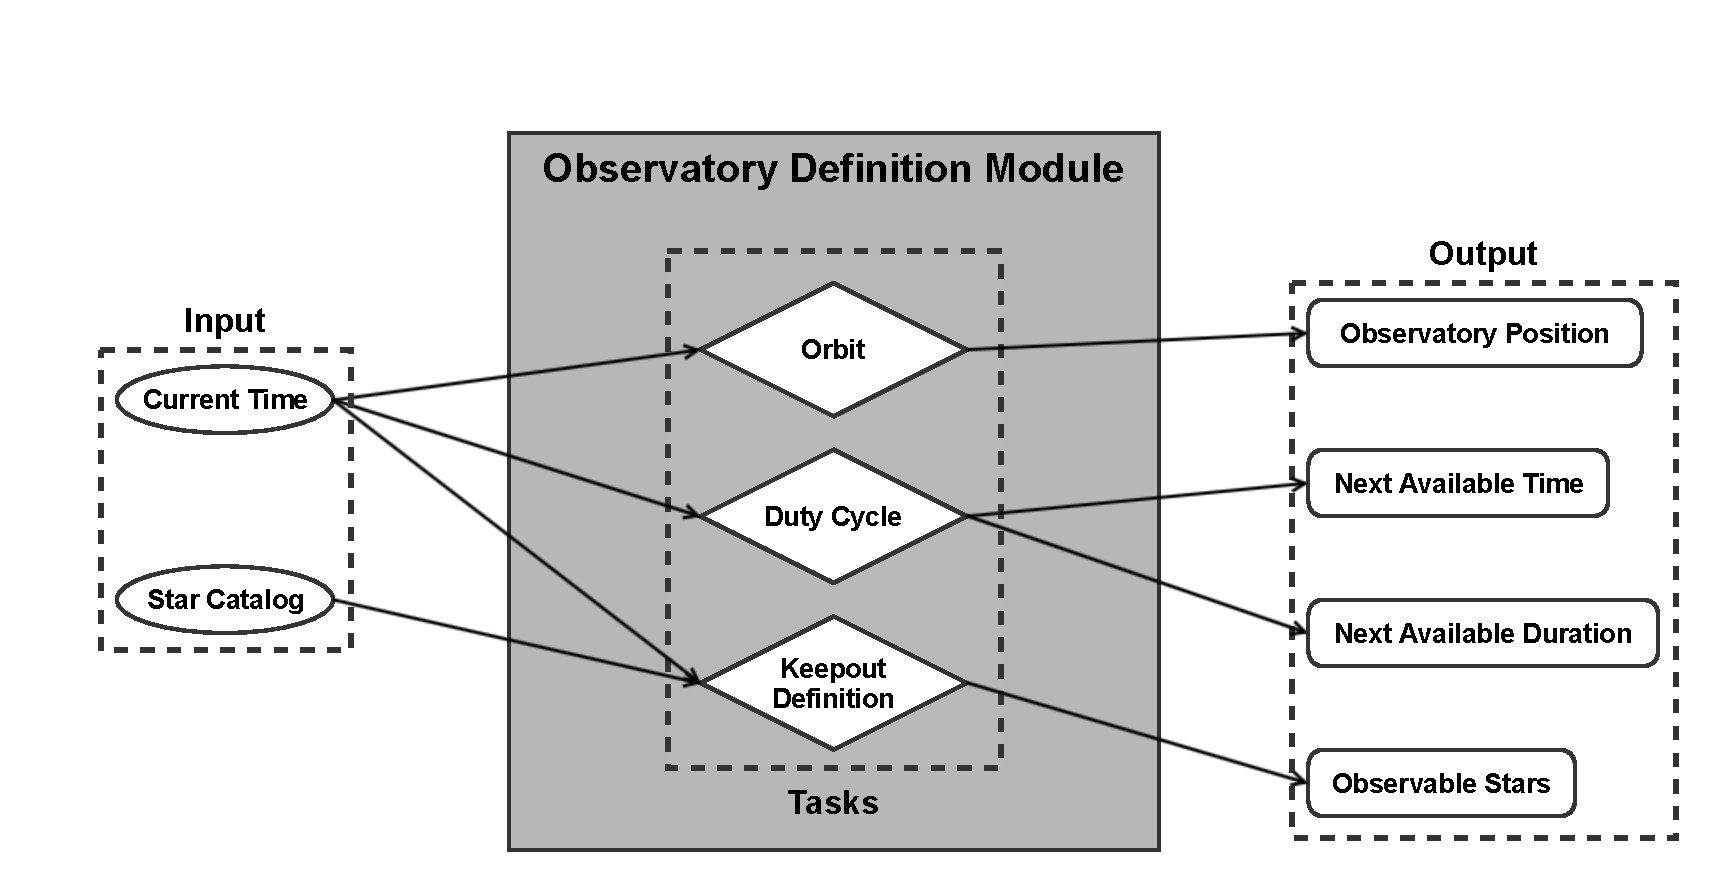
\includegraphics[width=\textwidth]{observatory2}
        \end{tabular}
    \end{center}
    \caption{\label{fig:observatory} Depiction of Observatory Definition module including inputs, tasks, and outputs.}
\end{figure}

\label{sec:observatorydefinition}
\subsubsection{Observatory Object Attribute Initialization Input/Output Description}

\subsubsection*{Inputs}
\begin{itemize}
    \item
    \begin{description}
        \item[User specification] \hfill \\
        Information from simulation specification JSON file organized into a Python dictionary. If the below key: value pairs are missing from the dictionary, the Observatory object attributes will be assigned the default values listed.
        \begin{description}
            \item specs["settling\_time"] \hfill \\
            Amount of time needed for observatory to settle after a repointing in $ days $. Default value is 1.
            \item specs["thrust"] \hfill \\
            Occulter slew thrust in $ mN $. Default value is 450.
            \item specs["slewIsp"] \hfill \\
            Occulter slew specific impulse in $ s $. Default value is 4160.
            \item specs["sc\_mass"] \hfill \\
            Occulter (maneuvering spacecraft) initial wet mass in $ kg $. Default value is 6000.
            \item specs["dryMass"] \hfill \\
            Occulter (maneuvering spacecraft) dry mass in $ kg $. Default value is 3400.
            \item specs["coMass"] \hfill \\
            Telescope (or non-maneuvering spacecraft) mass in $ kg $. Default value is 5800.
        \end{description}
    \end{description}
\end{itemize}

\subsubsection*{Outputs}
\begin{itemize}
    \item
    \begin{description}
        \item[Observatory.settling\_time] \hfill \\
        Amount of time needed for observatory to settle after a repointing (astropy unit object initially set in days)
        \item[Observatory.thrust] \hfill \\
        Occulter slew thrust (astropy unit object initially set in $ mN $)
        \item[Observatory.slewIsp] \hfill \\
        Occulter slew specific impulse (astropy unit object initially set in $ s $)
        \item[Observatory.sc\_mass] \hfill \\
        Occulter (maneuvering spacecraft) initial wet mass (astropy unit object initially set in $ kg $)
        \item[Observatory.dryMass] \hfill \\
        Occulter (maneuvering spacecraft) dry mass (astropy unit object initially set in $ kg $)
        \item[Observatory.coMass] \hfill \\
        Telescope (or non-maneuvering spacecraft) mass (astropy unit object initially set in $ kg $)
        \item[Observatory.kogood] \hfill \\
        Numpy array of Boolean values where True is a target unobstructed and observable in the keepout zone. Initialized to an empty array. This attribute is updated to the current mission time through the keepout task (see \ref{sec:keepouttask}).
        \item[Observatory.r\_sc] \hfill \\
        Observatory orbit position in HE reference frame. Initialized to numpy array as numpy.array([0., 0., 0.]) and associated with astropy unit object in $ km $. This attribute is updated to the orbital position of the observatory at the current mission time through the orbit task (see \ref{sec:orbittask}).
        \item[Observatory.flowRate] \hfill \\
        Slew flow rate derived from Observatory.thrust and Observatory.slewIsp (astropy unit object initially set in $ kg/day $)
        
    \end{description}
\end{itemize}

\subsubsection{Orbit Task Input/Output Description} \label{sec:orbittask}

\subsubsection*{Inputs}
\begin{itemize}
    \item
    \begin{description}
        \item[time.currenttimeAbs] \hfill \\
        Current absolute mission time (astropy \href{http://astropy.readthedocs.org/en/latest/time/index.html}{Time object}) from Time module see \ref{sec:currenttime} for definition
    \end{description}
\end{itemize}

\subsubsection*{Outputs}
\begin{itemize}
    \item
    \begin{description}
        \item[Observatory.r\_sc] \hfill \\
        Observatory orbit position in HE reference frame at current mission time (astropy unit object defined in $ km $)
    \end{description}
\end{itemize}

\subsubsection{Keepout Task Input/Output Description} \label{sec:keepouttask}

\subsubsection*{Inputs}
\begin{itemize}
    \item
    \begin{description}
        \item[time.currenttimeAbs] \hfill \\
        Current Absolute mission time (astropy Time object) from Time module see \ref{sec:currenttime} for definition
        \item[StarCatalog] \hfill \\
        Output of SC module. See \ref{sec:starcatalog} for definitions
    \end{description}
\end{itemize}

\subsubsection*{Outputs}
\begin{itemize}
    \item 
    \begin{description}
        \item[Observatory.kogood] \hfill \\
        List of Boolean values for each target at current mission time where True is when a target is unobstructed in the keepout zone and False is when a target cannot be observed due to obstructions in the keepout zone
    \end{description}
\end{itemize}



% PLANET PHYSICAL MODEL NEEDS UPDATING

\subsection{Planet Physical Model (PPM) NEEDS UPDATING}
The PPM module contains models of the light emitted or reflected by planets in the wavelength bands under investigation by the current mission simulation.  It takes as inputs the physical quantities sampled from the distributions in the PPD module and generates synthetic spectra (or band photometry, as appropriate).  The specific implementation of this module can vary greatly, and can be based on any of the many available planetary albedo, spectra and phase curve models.
\label{sec:planetphysicalmodel}

% TIME KEEPING WORK IN PROGRESS

\subsection{Time} 
The Time module is responsible for keeping track of the current mission time.  It encodes only the mission start time, the mission duration, and the current time within a simulation.  All functions in all modules requiring knowledge of the current time call functions or access parameters implemented within the Time module.  Internal encoding of time is implemented as the time from mission start (measured in days).  The Time module also provides functionality for converting between this time measure and standard measures such as Julian Day Number and UTC time.

TASKS:

\label{sec:time}
\subsubsection{Time Object Attribute Initialization Input/Output Description ORGANIZE LATER}

\subsubsection*{Inputs}
\begin{itemize}
    \item
    \begin{description}
        \item[User specification] \hfill \\
        Information from simulation specification JSON file organized into a Python dictionary. If the below key: value pairs are missing from the dictionary, the Time object attributes will be assigned the default values listed.
        \begin{description}
            \item specs["missionStart"] \hfill \\
            Mission start time in $ MJD $. Default value is 60634.
            \item specs["missionLife"] \hfill \\
            Total length of mission in $ days $. Default value is 2191.5.
        \end{description}
    \end{description}
\end{itemize}

\subsubsection*{Outputs}
\begin{itemize}
    \item
    \begin{description}
        \item[TimeKeeping.missionStart] \hfill \\
        Mission start time (astropy Time object initially defined in $ MJD $)
        \item[TimeKeeping.missionLife] \hfill \\
        Mission lifetime (astropy TimeDelta object initially defined in $ JD $ increments, where $ JD = MJD = 86400 s $)
        \item[TimeKeeping.currenttimeNorm] \hfill \\
        Current mission time normalized so that start date is 0 (astropy TimeDelta object initially defined in $ JD $ increments as above)
        \item[TimeKeeping.currenttimeAbs] \label{sec:currenttime}\hfill \\
        Current absolute mission time (astropy Time object initially defined in $ MJD $)
        \item[TimeKeeping.missionFinish] \hfill \\
        Mission completion date (astropy Time object initially defined in $ MJD $)

    \end{description}
\end{itemize}

% RULES NEEDS UPDATING

\subsection{Rules NEEDS UPDATING}
The Rules module contains additional constraints placed on the mission design not contained in other modules. These constraints are passed into the SS module to control the simulation. For example, a constraint in the Rules module could include prioritization of revisits to stars with detected exoplanets for characterization when possible. This rule would force the SS module to simulate observations for target stars with detected exoplanets when the OD module determines those stars are observable.

The Rules module also encodes the calculation of integration time for an observation.  This can be based on achieving a pre-determined signal to noise (SNR) metric (with various possible definitions), or via a probabilistic description.  This requires also defining a model for the background contribution due to all astronomical sources and especially due to zodiacal and exozodiacal light.

The duty cycle determines when during the mission timeline the observatory is allowed to perform planet-finding operations.  The duty cycle function takes the current mission time as input and outputs the next available time when exoplanet observations may begin or resume, along with the duration of the observational period. The outputs of this task are used in the SS module to determine when and how long exoplanet finding and characterization observations occur.  

TASKS:

\label{sec:rules}
\subsubsection{Rules Object Attribute Initialization Input/Output Description}

\subsubsection*{Inputs}
\begin{itemize}
    \item
    \begin{description}
        \item[User specification] \hfill \\
        Information from simulation specification JSON file organized into a Python dictionary. If the below key: value pairs are missing from the dictionary, the Rules object attributes will be assigned the default values listed.
        \begin{description}
            \item specs["FAP"] \hfill \\
            Detection false alarm probability. Default value is 0.01/1000.
            \item specs["MDP"] \hfill \\
            Missed detection probability. Default value is 0.001.
            \item specs["dutyCycle"] \hfill \\
            Observation duty cycle. Default value is 1.
            \item specs["intCutoff"] \hfill \\
            Maximum allowed integration time in $ days $. Default value is 50.
        \end{description}
    \end{description}
\end{itemize}

\subsubsection*{Outputs}
\begin{itemize}
    \item
    \begin{description}
        \item[Rules.FAP] \hfill \\
        Detection false alarm probability
        \item[Rules.MDP] \hfill \\
        Missed detection probability
        \item[Rules.dutyCycle] \hfill \\
        Observation duty cycle
        \item[Rules.intCutoff] \hfill \\
        Maximum allowed integration time (astropy unit object initially set to $ days $)
        \item[Rules.K] \hfill \\
        Threshold value determined by Rules.FAP
        \item[Rules.gamma] \hfill \\
        Threshold value determined by Rules.MDP
    \end{description}
\end{itemize}

% POST-PROCESSING NEEDS UPDATING

\subsection{Post-Processing (PP) NEEDS UPDATING}
The PP module encodes the effects of post-processing on the data gathered in a simulated observation, and the effects on the final contrast of the simulation.  The PP module is also responsible for determining whether a planet detection has occurred for a given observation, returning one of four possible states---true positive (real detection), false positive (false alarm), true negative (no detection when no planet is present) and false negative (missed detection).  These can be generated based solely on statistical modeling or by processing simulated images.
\label{sec:postprocessing}

% ZODIACAL LIGHT NEEDS UPDATING

\subsection{Zodiacal Light (ZL) NEEDS UPDATING}

TASKS: exozodi levels for each planetary system

\label{sec:zodiacallight}
\subsubsection{Zodiacal Light Object Attribute Initialization Input/Output Description ORGANIZE LATER}
\subsubsection*{Input}
\begin{itemize}
    \item
    \begin{description}
        \item[User specification] \hfill \\
        Information from simulation specification JSON file organized into a Python dictionary. If the below key: value pairs are missing from the dictionary, the Zodiacal Light object attributes will be assigned the default values listed.
        \begin{description}
            \item specs["exozodi"] \hfill \\
            Exo-zodi level in zodi
            \item specs["exozodiVar"] \hfill \\
            Exo-zodi variation (variance of log-normal distribution)
        \end{description}
    \end{description}
\end{itemize}

\subsubsection*{Output}
\begin{itemize}
    \item 
    \begin{description}
        \item[ZodiacalLight.exozodi] \hfill \\
        Exo-zodi level in zodi
        \item[ZodiacalLight.exozodiVar] \hfill \\
        Exo-zodi variation (variance of log-normal distribution)
    \end{description}
\end{itemize}

%%%%%%%%%%%%%%%%%%%%%%%%%%%%%%%%%%%%%%%%%%%%%%%%%%%%%%%%%%%%%%%%%%%%%%%%%
% SIMULATION MODULES
%%%%%%%%%%%%%%%%%%%%%%%%%%%%%%%%%%%%%%%%%%%%%%%%%%%%%%%%%%%%%%%%%%%%%%%%%

\section{Simulation Modules}
The simulation modules include Target List (TL), Simulated Universe (SU), Survey Simulation (SS) and Survey Ensemble (SE). These modules perform tasks which require inputs from one or more input modules as well as calling function implementations in other simulation modules.

% TARGET LIST NEEDS UPDATING

\subsection{Target List (TL) NEEDS UPDATING}
The TL module takes in information from the OSD, SC, PPD, and OD input modules and generates the target list for the simulated survey.  This list can either contain all of the targets where a planet with specified parameter ranges could be observed or a list of pre-determined targets such as in the case of a mission which only seeks to observe stars where planets are known to exist from previous surveys.  The final target list encodes all of the same information as is provided by the SC module.

\label{sec:targetlist}
\subsubsection{Target List Object Attribute Initialization Input/Output Description}
\subsubsection*{Inputs}
\begin{itemize}
    \item 
    \begin{description}
        \item[User specification] \hfill \\
        Information from simulation specification JSON file organized into a Python dictionary. If the below key: value pairs are missing from the dictionary, the Target List object attributes will be assigned the default values listed.
            \begin{description}
                \item specs["catalogname"] \hfill \\
                String containing name of desired SC module. Default is SC prototype module.
                \item specs["optsysname"] \hfill \\
                String containing name of desired OSD module. Default is OSD prototype module.
                \item specs["popname"] \hfill \\
                String containing name of desired PPD module. Default is PPD prototype module.
                \item specs["rulesname"] \hfill \\
                String containing name of desired Rules module. Default is Rules prototype module.
                \item specs["zodiname"] \hfill \\
                String containing name of desired ZL module. Default is ZL prototype module.
            \end{description}
        \item[StarCatalog] \hfill \\
        Output of SC module given by above specs["catalogname"] (see \ref{sec:starcatalog})
        \item[OpticalSys] \hfill \\
        Output of OSD module given by above specs["optsysname"] (see \ref{sec:opticalsystem})
        \item[PlanetPopulation] \hfill \\
        Output of PPD module given by above specs["popname"] (see \ref{sec:planetpopulation})
        \item[Rules] \hfill \\
        Output of Rules module given by above specs["rulesname"] (see \ref{sec:rules})
        \item[ZodiacalLight] \hfill \\
        Output of ZL module given by above specs["zodiname"] (see \ref{sec:zodiacallight})
    \end{description}
\end{itemize}

\subsubsection*{Outputs}
\begin{itemize}
    \item 
    \begin{description}
        \item[TargetList.(StarCatalog values)] \hfill \\
        Mission specific filtered star catalog values from SC module (see \ref{sec:starcatalog})
        \item[TargetList.OpticalSys] \hfill \\
        Output of OSD module (see \ref{sec:opticalsystem})
        \item[TargetList.PlanetPopulation] \hfill \\
        Output of PPD module (see \ref{sec:planetpopulation})
        \item[TargetList.Rules] \hfill \\
        Output of Rules module (see \ref{sec:rules})
        \item[TargetList.ZodiacalLight] \hfill \\
        Output of ZL module (see \ref{sec:zodiacallight})
        \item[TargetList.intTime] \hfill \\
        Numpy array of maximum integration time for each target star (astropy unit object initially defined in $ s $)
        \item[TargetList.MsEst] \hfill \\
        Approximate stellar mass in $ M_{sun} $
        \item[TargetList.MsTrue] \hfill \\
        Stellar mass with an error component included in $ M_{sun} $
    \end{description}
\end{itemize}

% SIMULATED UNIVERSE NEEDS UPDATING

\subsection{Simulated Universe (SU) NEEDS UPDATING}
The SU module takes as input the outputs of the TL simulation module to create a synthetic universe composed of the systems in the target list.  For each target, a planetary system is generated based on the statistics encoded in the PPD module, so that the overall planet occurrence and multiplicity rates are consistent with the provided distribution functions.  Physical parameters for each planet are similarly sampled from the input density functions.  This universe is encoded as a list where each entry corresponds to one element of the target list, and where the list entries are arrays of planet physical parameters.  In cases of empty planetary systems, the corresponding list entry contains a null array.

The SU module also takes as input the PPM module instance, so that it can return the specific spectra due to every simulated planet at an arbitrary observation time throughout the mission simulation.

TASKS:
\label{sec:simulateduniverse}
\subsubsection{Simulated Universe Object Attribute Initialization Input/Output Description}
\subsubsection*{Inputs}
\begin{itemize}
    \item 
    \begin{description}
        \item[User specification] \hfill \\
        Information from simulation specification JSON file organized into a Python dictionary. If the below key: value pairs are missing from the dictionary, the Simulated Universe object attributes will be assigned the default values listed.
            \begin{description}
                \item specs["targlistname"] \hfill \\
                String containing name of desired TL module. Default is TL prototype module.
                \item specs["planphysname"] \hfill \\
                String containing name of PPM module. Default is PPM prototype module.
            \end{description}
        \item[OpticalSys] \hfill \\
        Output of OSD module inherited from TL module (see \ref{sec:opticalsystem})
        \item[PlanetPopulation] \hfill \\
        Output of PPD module inherited from TL module (see \ref{sec:planetpopulation})
        \item[Rules] \hfill \\
        Output of Rules module inherited from TL module (see \ref{sec:rules})
        \item[ZodiacalLight] \hfill \\
        Output of ZL module inherited from TL module (see \ref{sec:zodiacallight})
        \item[TargetList] \hfill \\
        Output of TL module given by above specs["targlistname"] (see \ref{sec:targetlist})
        \item[PlanetPhysical] \hfill \\
        Output of PPM module given by above specs["planphysname"] (see \ref{sec:planetphysicalmodel})
    \end{description}
\end{itemize}

\subsubsection*{Outputs}
\begin{itemize}
    \item
    \begin{description}
        \item[SimulatedUniverse.OpticalSys] \hfill \\
        Output of OSD module (see \ref{sec:opticalsystem})
        \item[SimulatedUniverse.PlanetPopulation] \hfill \\
        Output of PPD module (see \ref{sec:planetpopulation})
        \item[SimulatedUniverse.Rules] \hfill \\
        Output of Rules module (see \ref{sec:rules})
        \item[SimulatedUniverse.ZodiacalLight] \hfill \\
        Output of ZL module (see \ref{sec:zodiacallight})
        \item[SimulatedUniverse.TargetList] \hfill \\
        Output of TL module (see \ref{sec:targetlist})
        \item[SimulatedUniverse.PlanetPhysical] \hfill \\
        Output of PPM module (see \ref{sec:planetphysicalmodel})
        \item[SimulatedUniverse.planInds] \hfill \\
        Numpy array containing indices of target list stars with planets
        \item[SimulatedUniverse.nPlans] \hfill \\
        Number of planetary systems
        \item[SimulatedUniverse.I] \hfill \\
        Numpy array containing list of inclination of planetary systems in degrees
    \end{description}
\end{itemize}

% SURVEY SIMULATION NEEDS UPDATING

\subsection{Survey Simulation (SS) NEEDS UPDATING}
The SS module takes as input the output of the SU simulation module and the Time, Rules, and PP input modules. This is the module that performs a specific simulation based on all of the input parameters and models. This module returns the mission timeline - an ordered list of simulated observations of various targets on the target list along with their outcomes.  The output also includes an encoding of the final state of the simulated universe (so that a subsequent simulation can start from where a previous simulation left off) and the final state of the observatory definition (so that post-simulation analysis can determine the percentage of volatiles expended, and other engineering metrics).

TASKS: 

\subsubsection{Survey Simulation Object Attribute Initialization Input/Output Description}
\subsubsection*{Inputs}
\begin{itemize}
    \item 
    \begin{description}
        \item[User specification] \hfill \\
        Information from simulation specification JSON file organized into a Python dictionary. If the below key: value pairs are missing from the dictionary, the Survey Simulation object attributes will be assigned the default values listed.
            \begin{description}
                \item specs["simuniname"] \hfill \\
                String containing name of desired SU module. Default is SU prototype module.
                \item specs["obsname"] \hfill \\
                String containing name of OD module. Default is OD prototype module.
                \item specs["timename"] \hfill \\
                String containing name of Time module. Default is Time prototype module
                \item specs["ppname"] \hfill \\
                String containing name of PP module. Default is PP prototype module
            \end{description}
        \item[OpticalSys] \hfill \\
        Output of OSD module inherited from SU module (see \ref{sec:opticalsystem})
        \item[PlanetPopulation] \hfill \\
        Output of PPD module inherited from SU module (see \ref{sec:planetpopulation})
        \item[Rules] \hfill \\
        Output of Rules module inherited from SU module (see \ref{sec:rules})
        \item[ZodiacalLight] \hfill \\
        Output of ZL module inherited from SU module (see \ref{sec:zodiacallight})
        \item[TargetList] \hfill \\
        Output of TL module inherited from SU module (see \ref{sec:targetlist})
        \item[PlanetPhysical] \hfill \\
        Output of PPM module inherited from SU module (see \ref{sec:planetphysicalmodel})
        \item[SimulatedUniverse] \hfill \\
        Output of SU module (see \ref{sec:simulateduniverse})
        \item[Observatory] \hfill \\
        Output of OD module (see \ref{sec:observatorydefinition})
        \item[TimeKeeping] \hfill \\
        Output of Time module (see \ref{sec:time})
        \item[PostProcessing] \hfill \\
        Output of PP module (see \ref{sec:postprocessing})
    \end{description}
\end{itemize}

\subsubsection*{Outputs}
\begin{itemize}
    \item
    \begin{description}
        \item[SurveySimulation.OpticalSys] \hfill \\
        Output of OSD module (see \ref{sec:opticalsystem})
        \item[SurveySimulation.PlanetPopulation] \hfill \\
        Output of PPD module (see \ref{sec:planetpopulation})
        \item[SurveySimulation.Rules] \hfill \\
        Output of Rules module (see \ref{sec:rules})
        \item[SurveySimulation.ZodiacalLight] \hfill \\
        Output of ZL module (see \ref{sec:zodiacallight})
        \item[SurveySimulation.TargetList] \hfill \\
        Output of TL module (see \ref{sec:targetlist})
        \item[SurveySimulation.PlanetPhysical] \hfill \\
        Output of PPM module (see \ref{sec:planetphysicalmodel})
        \item[SurveySimulation.SimulatedUniverse] \hfill \\
        Output of SU module (see \ref{sec:simulateduniverse})
        \item[SurveySimulation.Observatory] \hfill \\
        Output of OD module (see \ref{sec:observatorydefinition})
        \item[SurveySimulation.TimeKeeping] \hfill \\
        Output of Time module (see \ref{sec:time})
        \item[SurveySimulation.PostProcessing] \hfill \\
        Output of PP module (see \ref{sec:postprocessing})
        \item[SurveySimulation.visited] \hfill \\
        Numpy array giving number of observations for each star in the target list with indices corresponding to the target list. All are initialized to zero.
        \item[SurveySimulation.revisit\_list] \hfill \\
        Python list where each item gives index of star to revisit (corresponding to the target list) and mission time to revisit.
        \item[SurveySimulation.planPosTime] \hfill \\
        Numpy array giving current normalized time of each planet's position (astropy TimeDelta objects initially defined in $ JD $ increments as for TimeKeeping.currenttimeNorm, see \ref{sec:time}). All are initialized to zero as for TimeKeeping.currenttimeNorm. 
    \end{description}
\end{itemize}

% SURVEY ENSEMBLE NEEDS UPDATING

\subsection{Survey Ensemble (SE) NEEDS UPDATING}
The SE module's only task is to run multiple simulations.  While the implementation of this module is not at all dependent on a particular mission design, it can vary to take advantage of available parallel-processing resources.  As the generation of a survey ensemble is an embarrassingly parallel task---every survey simulation is fully independent and can be run as a completely separate process---significant gains in execution time can be achieved with parallelization.  The baseline implementation of this module contains a simple looping function that executes the desired number of simulations sequentially, as well as a locally parallelized version based on IPython Parallel.

\end{document}
